\subsubsection{Dịch vụ trò chuyện (conversation service) và Dịch vụ chatbot (chatbot service)}

Sơ đồ tổng quan về dịch vụ trò chuyện (conversation service) và dịch vụ chatbot (chatbot service):

\begin{figure}[H]
\centering
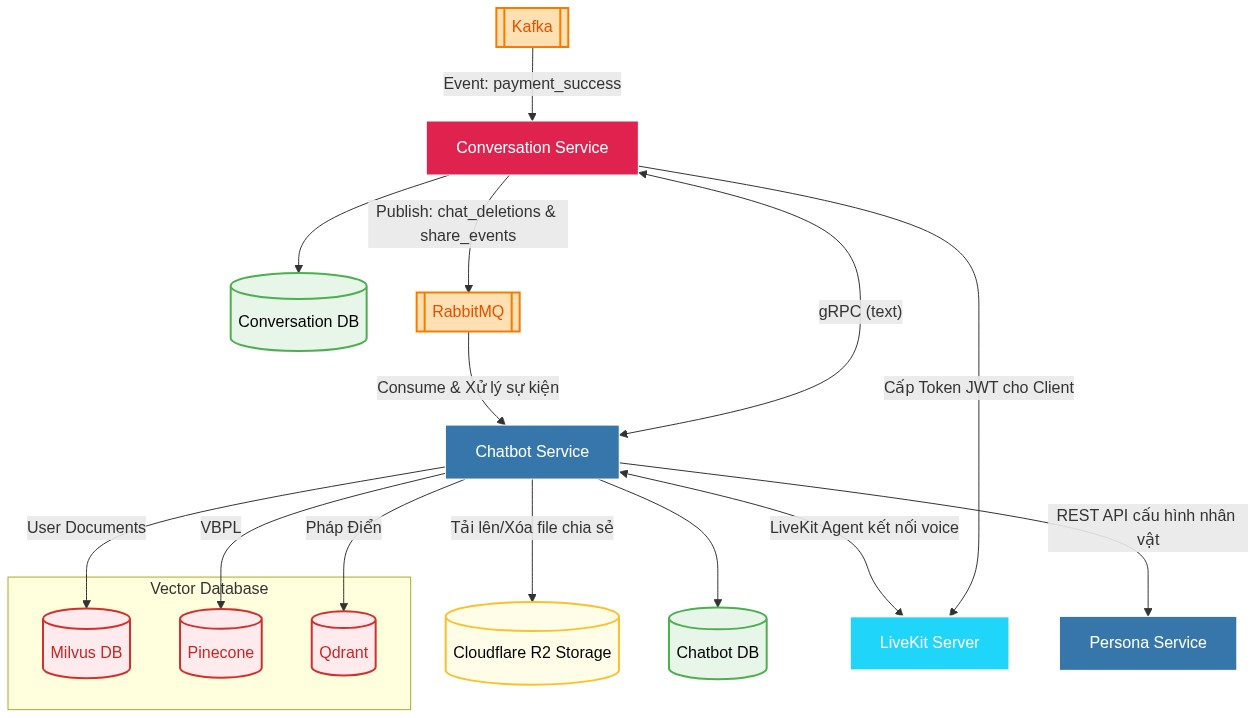
\includegraphics[width=0.95\textwidth]{pictures/conversation-and-chatbot-overview.png}
\caption{Sơ đồ tổng quan dịch vụ trò chuyện và dịch vụ chatbot}
\end{figure}

\paragraph{Dịch vụ trò chuyện (conversation service)}
Chịu trách nhiệm quản lý luồng giao tiếp giữa người dùng và hệ thống Agentic RAG. Dịch vụ này xử lý trực tiếp các cuộc trò chuyện văn bản theo cơ chế streaming, cấp phát token truy cập cho luồng giao tiếp giọng nói và cung cấp các tiện ích lưu trữ, chia sẻ trò chuyện.
Vì chức năng trò chuyện văn bản suy luận (reasoning) và trò chuyện bằng giọng nói chỉ dành riêng cho tài khoản VIP, nên dịch vụ trò chuyện (conversation service) thực hiện lắng nghe sự kiện thanh toán thành công từ Kafka, lưu lại thông tin vào CSDL và kiểm tra quyền VIP của người dùng hiện tại trước khi xử lý yêu cầu.

Các tính năng chính:
\begin{itemize}
\item \textbf{Khởi tạo trò chuyện}: Bắt đầu một luồng trò chuyện mới trong hệ thống.
\item \textbf{Cấp phát token thoại}: Cấp phát token bảo mật phục vụ kết nối đàm thoại bằng giọng nói với máy chủ LiveKit.
\item \textbf{Định tuyến tin nhắn}: Tiếp nhận tin nhắn từ người dùng và kết nối với dịch vụ chatbot (chatbot service) thông qua giao thức gRPC để xử lý thông tin.
\item \textbf{Xóa cuộc trò chuyện}: Hỗ trợ xóa mềm và lập lịch xóa dữ liệu sau khoảng thời gian.
\item \textbf{Quản lý thư mục}: Cho phép người dùng tạo các thư mục lưu trữ để phân loại và sắp xếp các cuộc trò chuyện.
\item \textbf{Đánh dấu và Ghi chú}: Đánh dấu một cuộc trò chuyện quan trọng và ghi chú các nội dung tóm tắt đi kèm.
\item \textbf{Chia sẻ trò chuyện}: Tạo ra một bản snapshot chia sẻ đoạn trò chuyện với người dùng khác.
\item \textbf{Đường dẫn chia sẻ}: Cung cấp URL công khai chứa tham số \texttt{shareId} và token bảo mật đi kèm. Chủ sở hữu đoạn chat có thể xem danh sách các liên kết đã tạo và thu hồi quyền truy cập bất cứ lúc nào.
\end{itemize}

\begin{figure}[H]
\centering
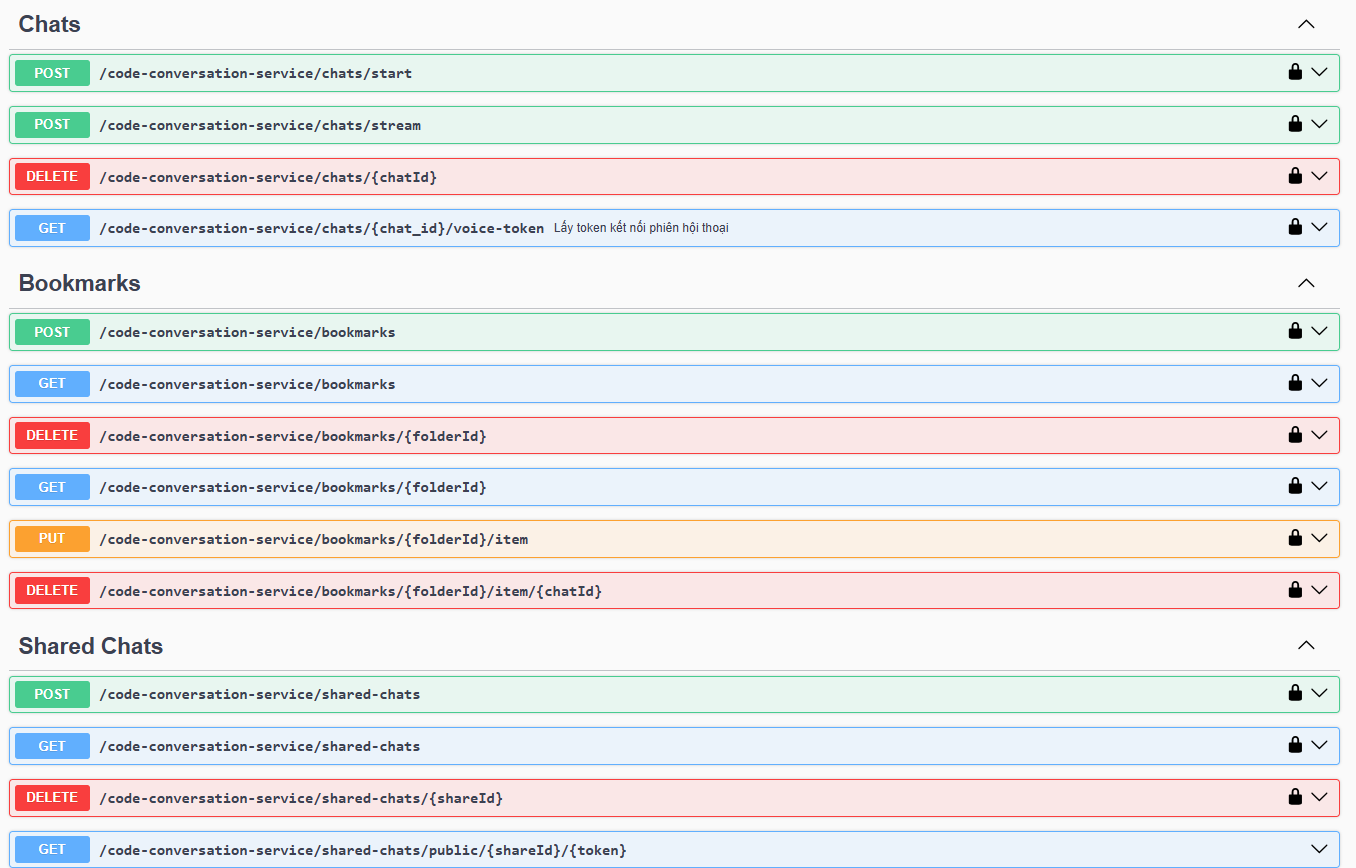
\includegraphics[width=0.95\textwidth]{pictures/conversation-swagger.png}
\caption{Tài liệu Swagger API dịch vụ trò chuyện}
\end{figure}

Sơ đồ trình tự kiểm duyệt nghiệp vụ khi xóa cuộc trò chuyện và chặn đứng việc chia sẻ cuộc trò chuyện đã bị xóa:

\begin{figure}[H]
\centering
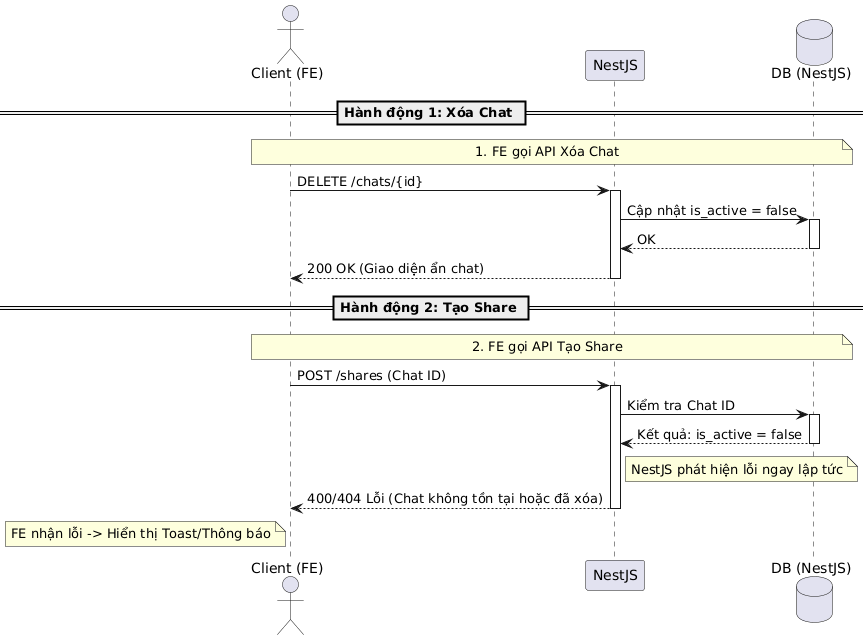
\includegraphics[width=0.85\textwidth]{pictures/delete-chat-validation-share.png}
\caption{Sơ đồ trình tự xóa cuộc trò chuyện và kiểm duyệt chia sẻ}
\end{figure}

\textbf{Chi tiết luồng xử lý và kiểm duyệt (Validation Logic):}
\begin{enumerate}
\item \textbf{Xóa cuộc trò chuyện (Delete Chat)}: Client gửi yêu cầu \texttt{DELETE /chats/\{id\}} đến dịch vụ trò chuyện (NestJS). Hệ thống tiến hành cập nhật trường trạng thái của cuộc trò chuyện trong Database thành \texttt{isActive = false} (thực hiện cơ chế xóa mềm - soft delete) và phản hồi \texttt{200 OK}. Lúc này, cuộc trò chuyện sẽ lập tức được ẩn đi trên giao diện người dùng.
\item \textbf{Kiểm duyệt tạo liên kết chia sẻ (Validate Share Link)}: Khi client gửi yêu cầu \texttt{POST /shares} (kèm theo \texttt{chat\_id}) để tạo link chia sẻ công khai, trước khi lưu bản ghi chia sẻ, \texttt{GenerateLinkShareCommandHandler} sẽ truy vấn thông tin cuộc trò chuyện từ Database dựa trên \texttt{chat\_id}. Nếu cuộc trò chuyện không tồn tại hoặc có trạng thái \texttt{isActive = false} (đã bị xóa mềm), hệ thống sẽ chặn đứng hành động ngay lập tức và ném ra lỗi \texttt{ChatNotFoundException} (trả về mã lỗi \texttt{400/404} cho client kèm theo thông báo lỗi chi tiết trên giao diện UI).
\end{enumerate}

Thông tin kiểm tra tự động Pull Request của dịch vụ trò chuyện trên GitHub:

\begin{figure}[H]
\centering
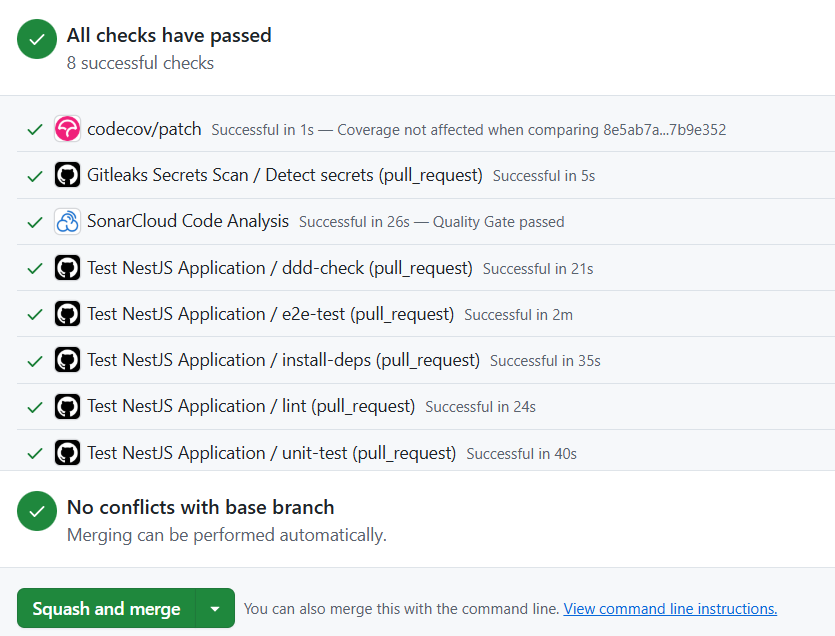
\includegraphics[width=0.8\textwidth]{pictures/conversation-PR-v2.png}
\caption{Kiểm tra Pull Request của dịch vụ trò chuyện trên GitHub}
\end{figure}

Quy trình chạy Test của dịch vụ trò chuyện trên GitHub Actions:

\begin{figure}[H]
\centering
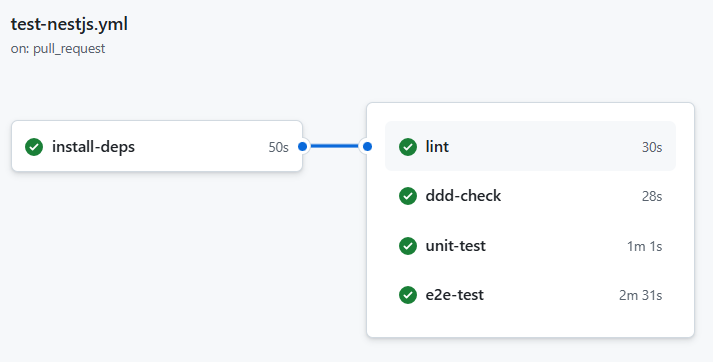
\includegraphics[width=0.95\textwidth]{pictures/conversation-lint.png}
\caption{Quy trình chạy Test của dịch vụ trò chuyện trên GitHub Actions}
\end{figure}

Quản lý di chuyển CSDL của dịch vụ trò chuyện:

\begin{figure}[H]
\centering
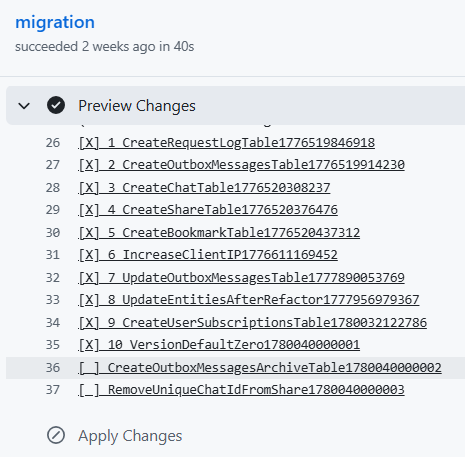
\includegraphics[width=0.95\textwidth]{pictures/conversation-database-migration.png}
\caption{Quản lý di chuyển CSDL dịch vụ trò chuyện}
\end{figure}

Cấu hình các bảng trong CSDL dịch vụ trò chuyện:

\begin{figure}[H]
\centering
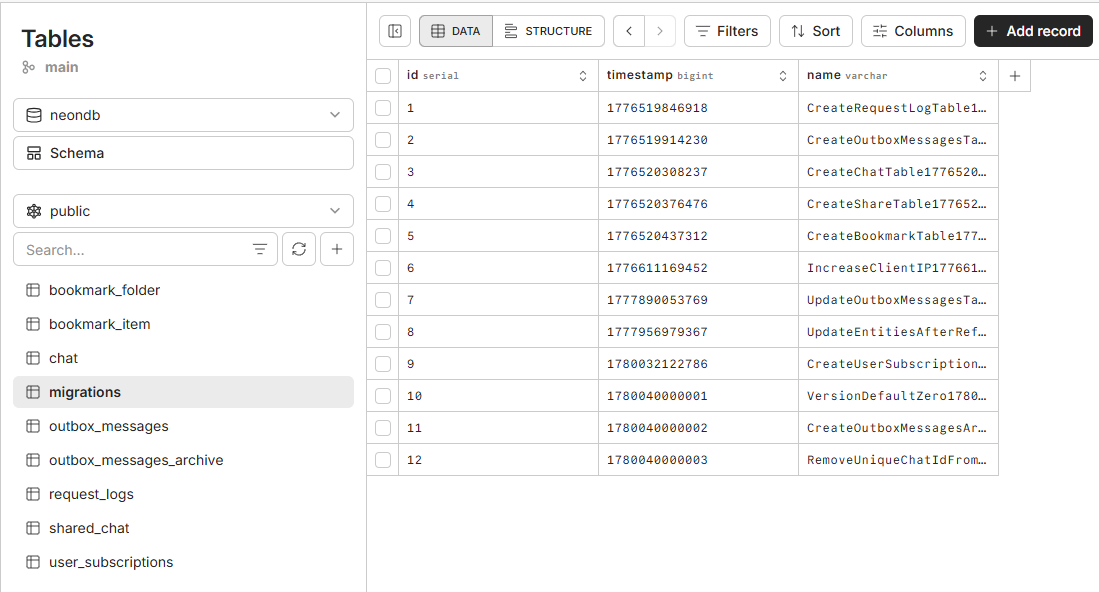
\includegraphics[width=0.95\textwidth]{pictures/conversation-database.png}
\caption{Cấu hình các bảng trong CSDL dịch vụ trò chuyện}
\end{figure}

\paragraph{Dịch vụ chatbot (chatbot service)}

% Mục đích:
Sử dụng các mô hình AI để xử lý và phản hồi thông minh các câu hỏi của người dùng.
Sau đó, lưu lại lịch sử trò chuyện và cung cấp các API truy xuất lịch sử,
thông tin suy luận chi tiết và nguồn tài liệu tham khảo của từng câu trả lời.
Dịch vụ chatbot lắng nghe RabbitMQ để thực hiện việc tạo và thu hồi các bản snapshot chia sẻ trò chuyện, đồng thời kết nối với LiveKit để vận hành đàm thoại giọng nói với người dùng.

\begin{figure}[H]
\centering
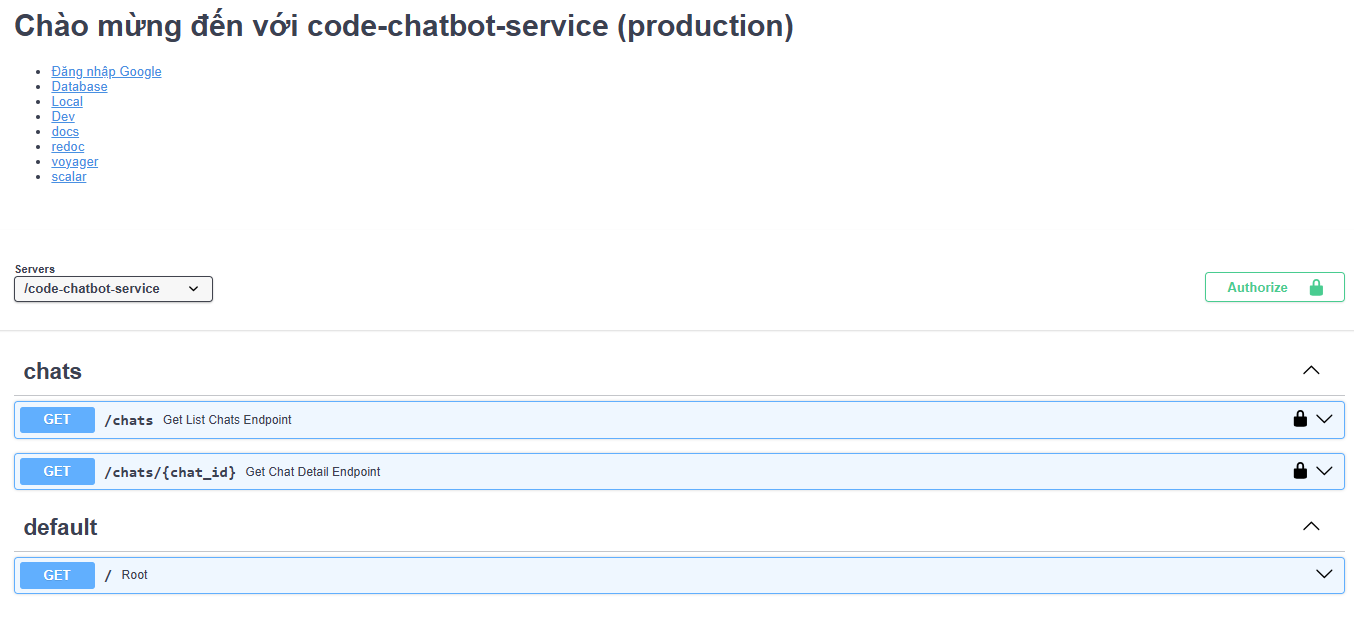
\includegraphics[width=0.99\textwidth]{pictures/chatbot-swagger.png}
\caption{Tài liệu Swagger API dịch vụ chatbot}
\end{figure}

Quản lý di chuyển CSDL của dịch vụ chatbot:

\begin{figure}[H]
\centering
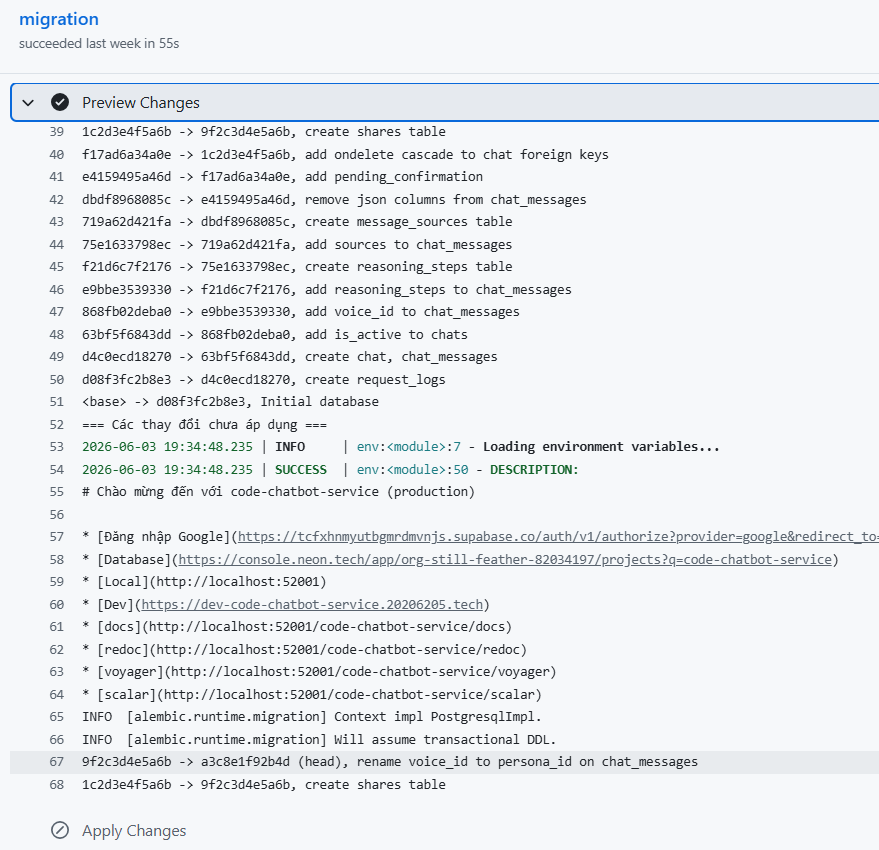
\includegraphics[width=0.9\textwidth]{pictures/chatbot-database-migration.png}
\caption{Quản lý di chuyển CSDL dịch vụ chatbot}
\end{figure}

Cơ cấu các bảng trong CSDL của dịch vụ chatbot:

\begin{figure}[H]
\centering
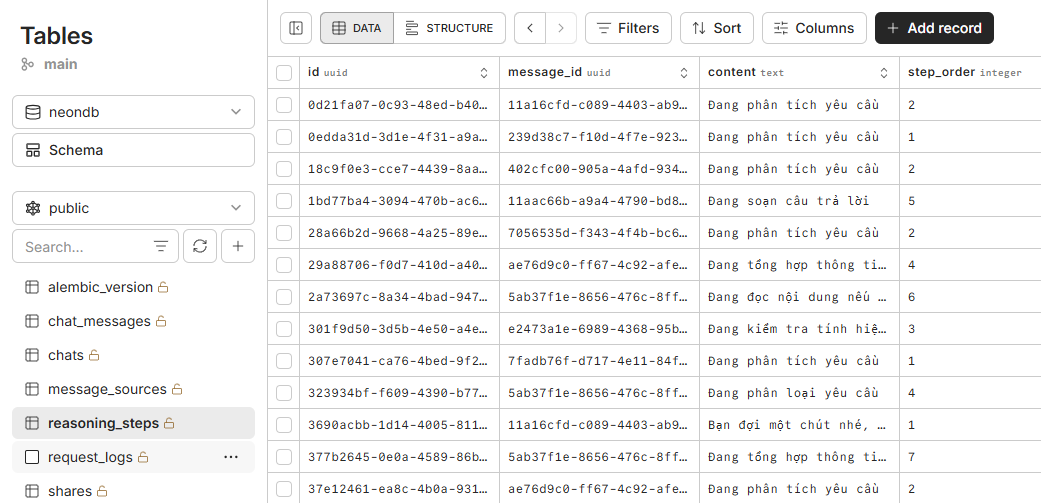
\includegraphics[width=0.95\textwidth]{pictures/chatbot-database.png}
\caption{Cấu hình các bảng trong CSDL chatbot}
\end{figure}

\paragraph{Hệ thống trao đổi thông điệp qua RabbitMQ (RabbitMQ Messaging)}

Hệ thống sử dụng \textbf{RabbitMQ} làm Message Broker để thực hiện các giao tiếp bất đồng bộ, đáng tin cậy giữa \textbf{dịch vụ trò chuyện (NestJS)} và \textbf{dịch vụ chatbot (Python)}. Các tên hàng đợi được tiền tố hóa tự động theo môi trường (\texttt{dev\_}, \texttt{test\_}, \texttt{prod\_}) dựa trên cấu hình hệ thống.

\subparagraph{Danh sách các hàng đợi trong hệ thống}

\begin{itemize}
\item \textbf{\texttt{[prefix]\_chat\_deletions}}: Nhận yêu cầu xóa mềm (soft delete) lịch sử chat từ phía người dùng (Durable: \texttt{true}).

\item \textbf{\texttt{[prefix]\_share\_generated}}: Yêu cầu tạo trang chia sẻ trò chuyện công khai (đóng gói JSONL và tải lên Cloudflare R2).

\item \textbf{\texttt{[prefix]\_share\_generated\_retry}}: Hàng đợi trung gian để xử lý lại (retry) khi gặp lỗi lệch thứ tự sự kiện (out of order). Cấu hình độ trễ cố định \texttt{x-message-ttl = 20s} trước khi gửi trả lại queue chính.

\item \textbf{\texttt{[prefix]\_share\_generated\_dlq}}: Dead Letter Queue nhận thông điệp tạo share thất bại hoàn toàn sau \texttt{MAX\_RETRY\_COUNT = 5} lần thử lại.

\item \textbf{\texttt{[prefix]\_share\_upload\_completed}}: Báo cáo kết quả đóng gói và upload file chia sẻ từ Python về lại NestJS.

\item \textbf{\texttt{[prefix]\_share\_upload\_completed\_dlq}}: Dead Letter Queue nhận thông điệp báo cáo kết quả upload bị xử lý thất bại ở NestJS.

\item \textbf{\texttt{[prefix]\_share\_revoked}}: Nhận yêu cầu thu hồi link chia sẻ, tiến hành xóa file tương ứng trên Cloudflare R2 và cập nhật DB (Durable: \texttt{true}).
\end{itemize}

% \begin{figure}[H]
% \centering
% 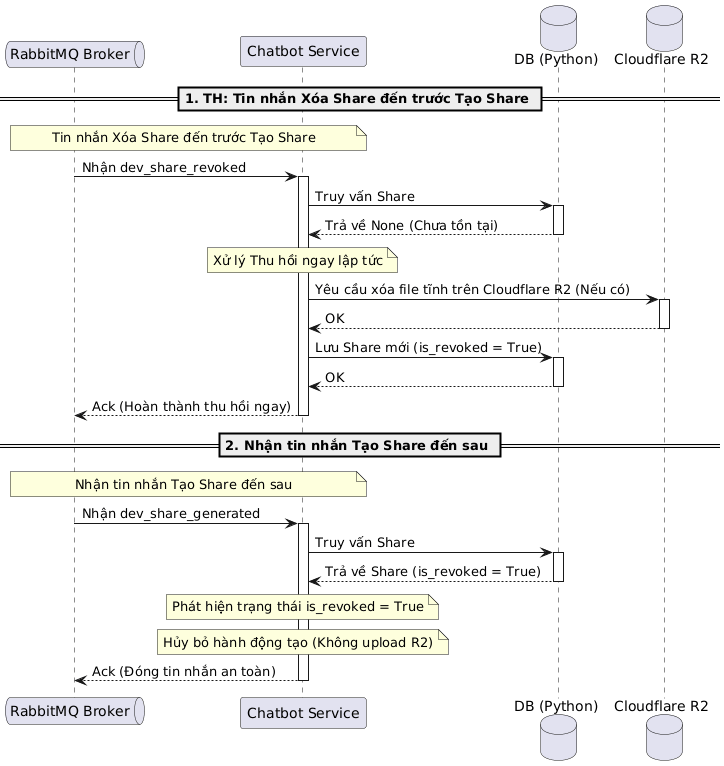
\includegraphics[width=0.95\textwidth]{pictures/share-out-of-order.png}
% \caption{Danh sách các hàng đợi trong hệ thống}
% \end{figure}

% \subparagraph{Cấu trúc dữ liệu và Luồng xử lý sự kiện}

\textbf{Sự kiện Xóa trò chuyện}
\begin{itemize}
\item \textbf{Hàng đợi}: \texttt{[prefix]\_chat\_deletions}
\item \textbf{Bên xuất bản}: \texttt{code-conversation-service} (NestJS)
\item \textbf{Bên tiêu thụ}: \texttt{code-chatbot-service} (Python)

\begin{table}[H]
\centering
\begin{tabular}{|l|l|l|}
\hline
\textbf{Thuộc tính} & \textbf{Kiểu dữ liệu} & \textbf{Mô tả} \\ \hline
\texttt{chat\_id} & String & Mã ID cuộc trò chuyện cần xóa \\ \hline
\texttt{user\_id} & String & Mã ID người dùng sở hữu cuộc trò chuyện \\ \hline
\texttt{version} & Number & Phiên bản sự kiện để kiểm tra thứ tự \\ \hline
\end{tabular}
\caption{Cấu trúc dữ liệu sự kiện ChatDeletedEvent}
\end{table}

\end{itemize}

\textbf{Sự kiện Yêu cầu chia sẻ (Share Generated Event)}
\begin{itemize}
\item \textbf{Hàng đợi}: \texttt{[prefix]\_share\_generated}
\item \textbf{Bên xuất bản}: \texttt{code-conversation-service} (NestJS)
\item \textbf{Bên tiêu thụ}: \texttt{code-chatbot-service} (Python)

\begin{table}[H]
\centering
\begin{tabular}{|l|l|l|}
\hline
\textbf{Thuộc tính} & \textbf{Kiểu dữ liệu} & \textbf{Mô tả} \\ \hline
\texttt{share\_id} & String & ID duy nhất của liên kết chia sẻ \\ \hline
\texttt{chat\_id} & String & ID cuộc trò chuyện được chia sẻ \\ \hline
\texttt{user\_id} & String & ID người dùng tạo chia sẻ \\ \hline
\texttt{version} & Number & Phiên bản sự kiện \\ \hline
\texttt{last\_message\_id} & String & ID tin nhắn cuối cùng \\ \hline
\end{tabular}
\caption{Cấu trúc dữ liệu sự kiện ChatSharedEvent}
\end{table}

\item \textbf{Cơ chế xử lý lệch thứ tự (Out-of-Order)}:
Consumer Python so sánh phiên bản sự kiện nhận được
với phiên bản hiện tại trong DB.
Nếu \texttt{event\_version == current\_version + 1},
tiến hành đóng gói lịch sử chat,
upload R2 và gửi kết quả về NestJS.
Nếu \texttt{event\_version <= current\_version},
bỏ qua vì đã xử lý.
Nếu \texttt{event\_version > current\_version + 1},
sự kiện đến sai thứ tự,
ném ra ngoại lệ \texttt{OutOfOrderException}
để đưa tin nhắn vào \texttt{retry}
tạm chờ 20 giây trước khi thử lại.
Sau 5 lần thất bại liên tục sẽ bị chuyển vào
DLQ và gửi cảnh báo về hệ thống.
\end{itemize}

\textbf{Sự kiện Thu hồi liên kết (Share Revoked Event)}
\begin{itemize}
\item \textbf{Hàng đợi}: \texttt{[prefix]\_share\_revoked}
\item \textbf{Bên xuất bản}: \texttt{code-conversation-service} (NestJS)
\item \textbf{Bên tiêu thụ}: \texttt{code-chatbot-service} (Python)

\begin{table}[H]
\centering
\begin{tabular}{|l|l|l|}
\hline
\textbf{Thuộc tính} & \textbf{Kiểu dữ liệu} & \textbf{Mô tả} \\ \hline
\texttt{share\_id} & String & ID liên kết chia sẻ cần thu hồi \\ \hline
\texttt{file\_url} & String & URL tệp tin JSONL cần xóa trên Cloudflare R2 \\ \hline
\texttt{version} & Number & Phiên bản sự kiện (thường là phiên bản kế tiếp) \\ \hline
\end{tabular}
\caption{Cấu trúc dữ liệu sự kiện ShareRevokedEvent}
\end{table}

\item \textbf{Cơ chế xử lý}: Xóa tệp tin trên Cloudflare R2, đánh dấu \texttt{is\_revoked = True} trong DB. Hỗ trợ cơ chế tự động gửi lại hàng đợi chính (requeue) nếu phát hiện sự kiện đến lệch thứ tự (revoke đến trước khi generate kịp ghi DB).
\end{itemize}

\textbf{Sự kiện Hoàn tất Upload (Share Upload Completed Event)}
\begin{itemize}
\item \textbf{Hàng đợi}: \texttt{[prefix]\_share\_upload\_completed}
\item \textbf{Bên xuất bản}: \texttt{code-chatbot-service} (Python)
\item \textbf{Bên tiêu thụ}: \texttt{code-conversation-service} (NestJS)

\begin{table}[H]
\centering
\begin{tabular}{|l|l|l|}
\hline
\textbf{Thuộc tính} & \textbf{Kiểu dữ liệu} & \textbf{Mô tả} \\ \hline
\texttt{share\_id} & String & ID liên kết chia sẻ tương ứng \\ \hline
\texttt{file\_url} & String & URL tệp tin JSONL \\ \hline
\texttt{is\_success} & Boolean & Trạng thái thành công \\ \hline
\end{tabular}
\caption{Cấu trúc dữ liệu sự kiện ShareProcessStatusEvent}
\end{table}

\item \textbf{Cơ chế xử lý}: NestJS nhận thông điệp sẽ tiến hành cập nhật trạng thái của bản ghi chia sẻ thành công hoặc thất bại trong DB (sử dụng Manual Ack để đảm bảo không bị mất dữ liệu).
\end{itemize}

\textbf{Xử lý lệch thứ tự sự kiện tạo chia sẻ và thu hồi chia sẻ}
\begin{itemize}
\item \textbf{Tình huống}: Người dùng vừa tạo chia sẻ và lập tức thực hiện thu hồi chia sẻ đó.
Do tính chất bất đồng bộ của Message Broker,
sự kiện Thu hồi chia sẻ (\texttt{share\_revoked})
có thể đến Python worker \textbf{trước} sự kiện tạo chia sẻ
(\texttt{share\_generated}).
\item \textbf{Cơ chế kiểm tra trạng thái lũy đẳng}:
Vì việc thu hồi liên kết thường liên quan đến vấn đề
rò rỉ thông tin nhạy cảm của người dùng,
nghiệp vụ yêu cầu lệnh thu hồi
phải được thực hiện
\textbf{ngay lập tức và ưu tiên cao nhất}.
Do đó, hệ thống không áp dụng cơ chế tuần tự
kiểm tra version phức tạp mà
sử dụng cờ trạng thái \texttt{is\_revoked}
để triệt tiêu sự kiện.
\end{itemize}

\begin{figure}[H]
\centering
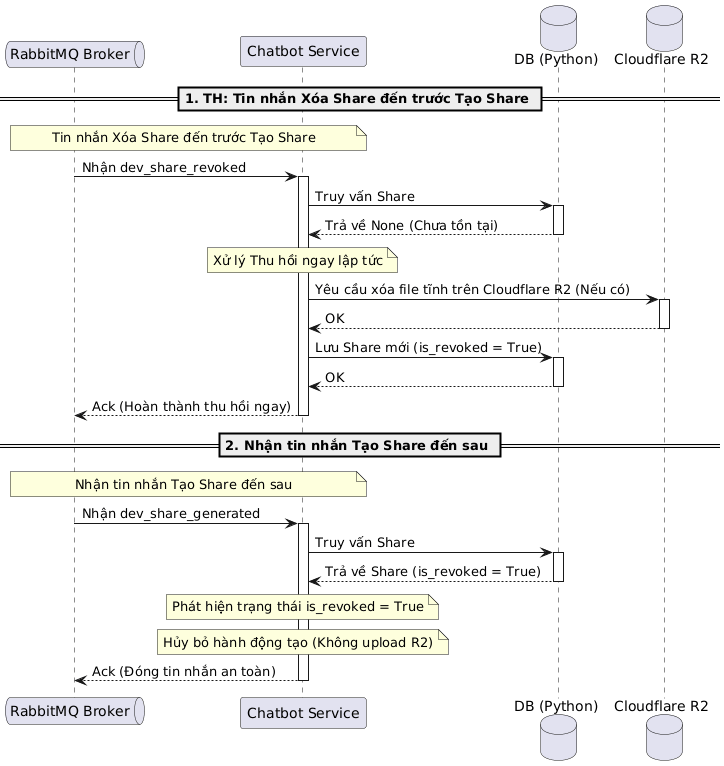
\includegraphics[width=0.99\textwidth]{pictures/share-out-of-order.png}
\caption{Sơ đồ xử lý lệch thứ tự tạo và thu hồi chia sẻ}
\end{figure}

\begin{enumerate}
\item \textbf{Khi sự kiện Thu hồi chia sẻ đến trước}:
Python kiểm tra trạng thái trong DB (chưa có bản ghi nào), tiến hành gọi xóa tệp tin trên Cloudflare R2 (nếu đã được tạo trước đó), lưu bản ghi chia sẻ vào DB với trạng thái \texttt{is\_revoked = True} và phản hồi \texttt{Ack} để hoàn thành tin nhắn.
\item \textbf{Khi sự kiện Tạo chia sẻ đến sau}:
Python kiểm tra DB và phát hiện bản ghi đã tồn tại với trạng thái \texttt{is\_revoked = True}. Khi đó, áp dụng \textbf{cơ chế triệt tiêu sự kiện (Event Cancellation)}: lập tức bỏ qua (drop) hoàn toàn hành động tạo và upload tệp lên R2 để bảo vệ tuyệt đối dữ liệu nhạy cảm của người dùng, sau đó gửi \texttt{Ack} để đóng tin nhắn một cách an toàn.
\end{enumerate}

% \textbf{Thiết lập hàng đợi ưu tiên (Priority Queue) trên RabbitMQ}

% Để đảm bảo các thông điệp thu hồi khẩn cấp được đẩy lên xử lý trước trong trường hợp hàng đợi bị nghẽn (backlog), hệ thống hỗ trợ tích hợp \textbf{Priority Queue}:
% \begin{enumerate}
% \item \textbf{Khai báo hàng đợi hỗ trợ ưu tiên}: Khi khởi tạo queue trên RabbitMQ, gán đối số cấu hình mức ưu tiên.
% % cao nhất (khuyến nghị tối đa là 10 để tránh tốn tài nguyên RAM/CPU):
% % \begin{verbatim}
% % channel.queue_declare(
% % queue='[prefix]_share_events_queue',
% % arguments={'x-max-priority': 10}
% % )
% % \end{verbatim}
% \item \textbf{Gửi sự kiện kèm mức độ ưu tiên (Producer)}: Sự kiện thu hồi chia sẻ (\texttt{share\_revoked}) được gửi với độ ưu tiên khẩn cấp (\texttt{priority = 10}). Sự kiện tạo chia sẻ (\texttt{share\_generated}) được gửi với độ ưu tiên bình thường (\texttt{priority = 1}).
% \item \textbf{Cấu hình cho consumer}: Thiết lập thuộc tính \texttt{prefetch\_count = 1} trên consumer để bắt buộc RabbitMQ chỉ gửi đúng 1 thông điệp tại một thời điểm cho worker. Điều này giúp hàng đợi có cơ hội sắp xếp và đẩy các tin nhắn có độ ưu tiên cao (\texttt{priority = 10}) lên xử lý trước.
% \end{enumerate}

\textbf{Luồng xử lý hàng đợi thư chết (DLQ) kết hợp cảnh báo Telegram}
\begin{itemize}
\item \textbf{Mục đích}: Khi một tin nhắn gặp lỗi xử lý lặp đi lặp lại nhiều lần (lỗi logic, lỗi kết nối CSDL kéo dài, lỗi phân tích cú pháp dữ liệu), hệ thống cần cô lập tin nhắn đó để tránh làm nghẽn hàng đợi chính, đồng thời phát cảnh báo tức thời cho đội ngũ vận hành (Developers/DevOps).
\item \textbf{Quy trình hoạt động}: Sự kết hợp giữa cơ chế Dead Letter Queue (DLQ) của RabbitMQ và Telegram Bot API được thực hiện như sau:
\end{itemize}

\begin{figure}[H]
\centering
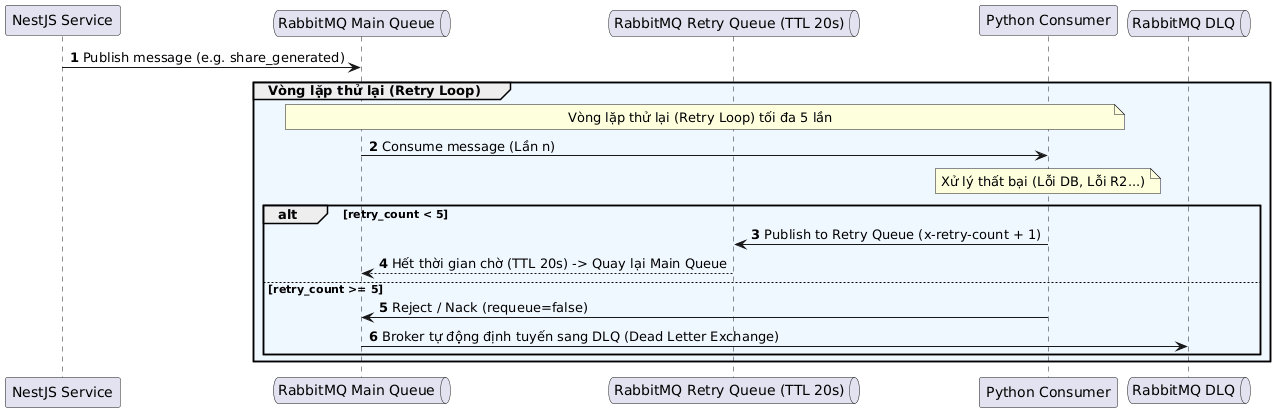
\includegraphics[width=0.99\textwidth]{pictures/dlq-telegram-alert-step1.png}
\caption{Sơ đồ vòng lặp thử lại (Retry Loop)}
\end{figure}

\begin{figure}[H]
\centering
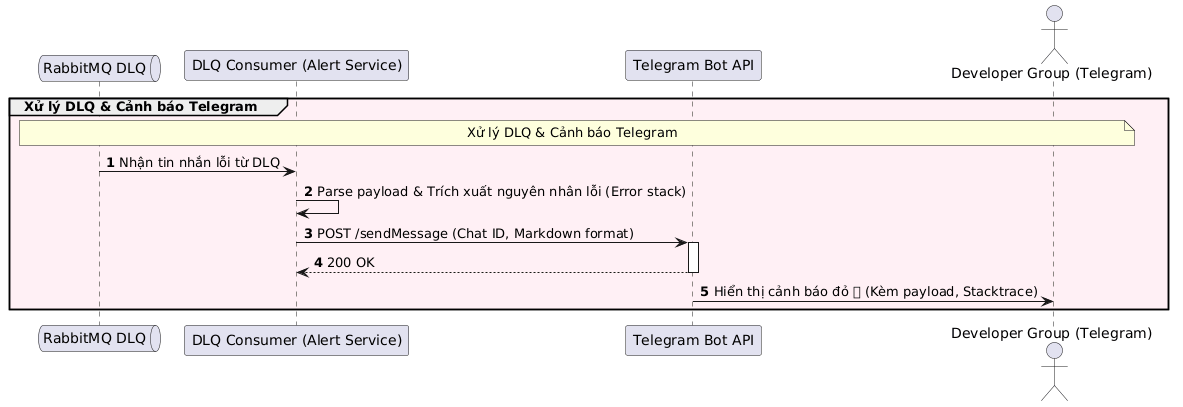
\includegraphics[width=0.99\textwidth]{pictures/dlq-telegram-alert-step2.png}
\caption{Sơ đồ xử lý DLQ và cảnh báo Telegram}
\end{figure}

\begin{enumerate}
\item \textbf{Ghi nhận và Thử lại (Retry Loop)}: Khi consumer (Python/NestJS) xử lý tin nhắn thất bại, tin nhắn sẽ được gửi sang hàng đợi Retry với độ trễ (TTL) cố định là 20 giây, đồng thời số lần thử lại (\texttt{x-retry-count}) được lưu và tăng dần trong header của tin nhắn.
\item \textbf{Chuyển sang DLQ}: Sau khi thử lại thất bại quá số lần quy định (\texttt{MAX\_RETRY\_COUNT = 5}), consumer sẽ từ chối tin nhắn không điều kiện (\texttt{message.reject(requeue=False)}). RabbitMQ sẽ tự động chuyển hướng tin nhắn này sang hàng đợi thư chết tương ứng (\texttt{\_dlq}) dựa trên cấu hình \texttt{x-dead-letter-routing-key} lúc khởi tạo queue.
\item \textbf{Tiêu thụ DLQ và Cảnh báo}: Một consumer chuyên biệt (\texttt{process\_share\_generated\_dlq}) sẽ lắng nghe hàng đợi DLQ. Khi có tin nhắn đi vào DLQ, consumer này sẽ trích xuất thông tin lỗi, payload của sự kiện, thời gian xảy ra sự cố và gửi yêu cầu HTTP POST tới Telegram Bot API để thông báo tức thời cho đội ngũ vận hành.
\end{enumerate}

\subparagraph{Xử lý concurrency khi Tạo Share và Xóa Chat đồng thời (Concurrency \& Snapshot Architecture)}

Trong thực tế vận hành, người dùng có thể thực hiện thao tác tạo liên kết chia sẻ (Share) và ngay lập tức xóa cuộc trò chuyện (Delete Chat). Lúc này, cơ chế Outbox sẽ đẩy đồng thời hai sự kiện \texttt{share\_generated} và \texttt{chat\_deleted} vào RabbitMQ. Để giải quyết bài toán Race Condition (xung đột tài nguyên) khi thứ tự xử lý trên RabbitMQ không cố định, hệ thống áp dụng mẫu kiến trúc \textbf{Snapshot/Static Generation}:

\textbf{Cơ chế hoạt động chi tiết:}
\begin{itemize}
\item \textbf{Không phụ thuộc vào trạng thái hoạt động của Chat:} Khi NestJS hoặc Python nhận sự kiện xóa chat, họ chỉ thực hiện \textbf{xóa mềm (soft delete)} bằng cách cập nhật trường \texttt{is\_active = False} trong CSDL. Bản ghi và dữ liệu tin nhắn vẫn tồn tại vật lý trong database.
\item \textbf{Tạo Snapshot tĩnh (Static Generation):} Dù sự kiện \texttt{chat\_deleted} có được xử lý trước sự kiện \texttt{share\_generated} trên Python worker, Python vẫn có thể truy vấn đầy đủ nội dung lịch sử chat đã xóa mềm từ database để đóng gói thành tệp JSONL tĩnh và tải lên Cloudflare R2.
\item \textbf{Tính độc lập của liên kết chia sẻ:}
Sau khi upload thành công lên Cloudflare R2,
trogn CSDL sẻ cập nhật thông tin liên kết đến tệp này.
Khi người nhận xem liên kết chia sẻ,
dịch vụ sẽ lấy thông tin tệp R2 từ CSDL và tải xuống xử lý.
% Frontend sẽ fetch trực tiếp tệp tĩnh từ R2 (qua CDN) mà không cần truy vấn vào database gốc (Neon) hay đi qua NestJS.
Nghiệp vụ chấp nhận trạng thái
% "Có liên kết chia sẻ hoạt động nhưng cuộc trò chuyện gốc đã bị xóa".
\enquote{Có liên kết chia sẻ hoạt động nhưng cuộc trò chuyện gốc đã bị xóa}.
Nếu muốn thu hồi sẽ có API khác thực hiện thu hồi chia sẻ.
\end{itemize}

\begin{figure}[H]
\centering
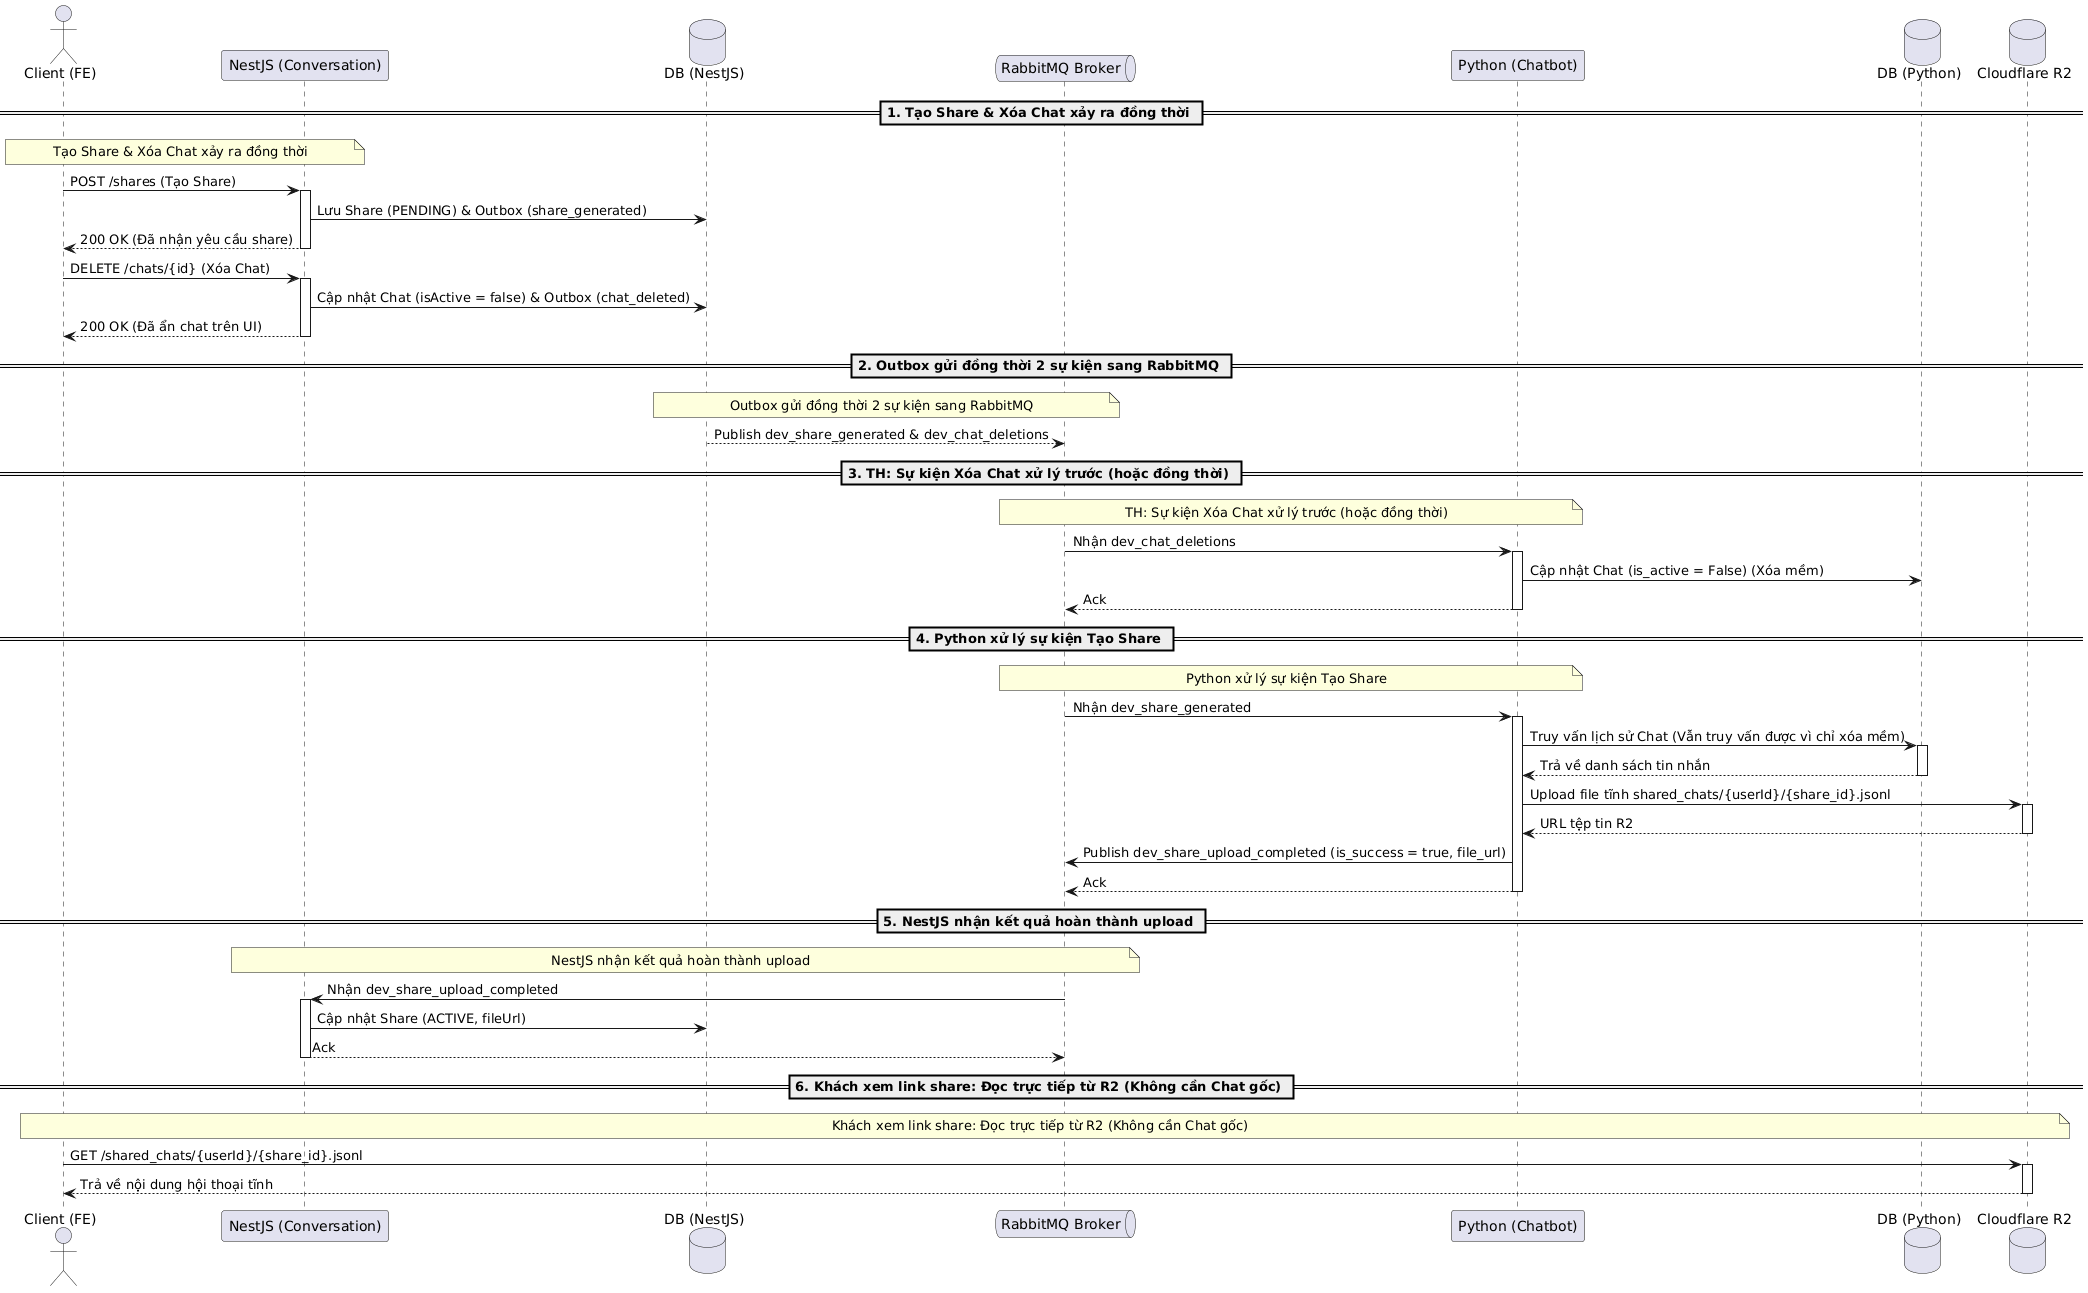
\includegraphics[width=0.99\textwidth]{pictures/share-concurrency-handling.png}
\caption{Sơ đồ xử lý đồng thời tạo share và xóa chat}
\end{figure}

Kết quả các tệp tin chia sẻ
trò chuyện lưu trữ
trên Cloudflare R2:

\begin{figure}[H]
\centering
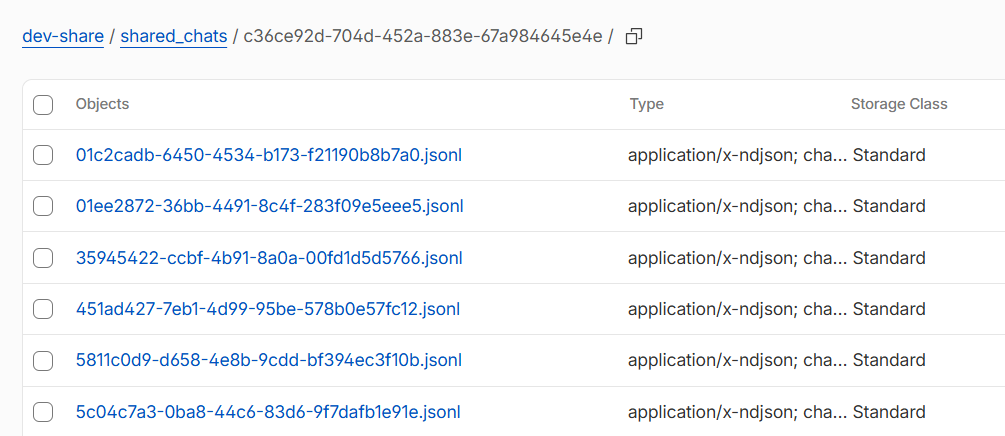
\includegraphics[width=0.99\textwidth]{pictures/r2chat.png}
\caption{Lưu trữ các tệp tin chia sẻ trên Cloudflare R2}
\end{figure}

\paragraph{Chi tiết chức năng đàm thoại giọng nói (Voice Agent)}

Hệ thống thiết lập các bộ chuyển đổi (Adapters) cho phép kết nối linh hoạt với nhiều nhà cung cấp mô hình ngôn ngữ (Groq, Ollama và NVIDIA) có hỗ trợ gọi công cụ (Tool Calling) để đảm bảo tính sẵn sàng cao của hệ thống.
AI Agent tích hợp sẵn công cụ lấy thông tin nhân vật (Get Persona) và công cụ gọi luồng xử lý LangGraph để phản hồi câu hỏi.
Hệ thống hỗ trợ tự động chuyển đổi công cụ TTS giữa ElevenLabs, Edge TTS và Piper TTS để đáp ứng linh hoạt theo cấu hình nhân vật của người dùng.

Sơ đồ tổng quan luồng tích hợp LiveKit đàm thoại giọng nói:

\begin{figure}[H]
\centering
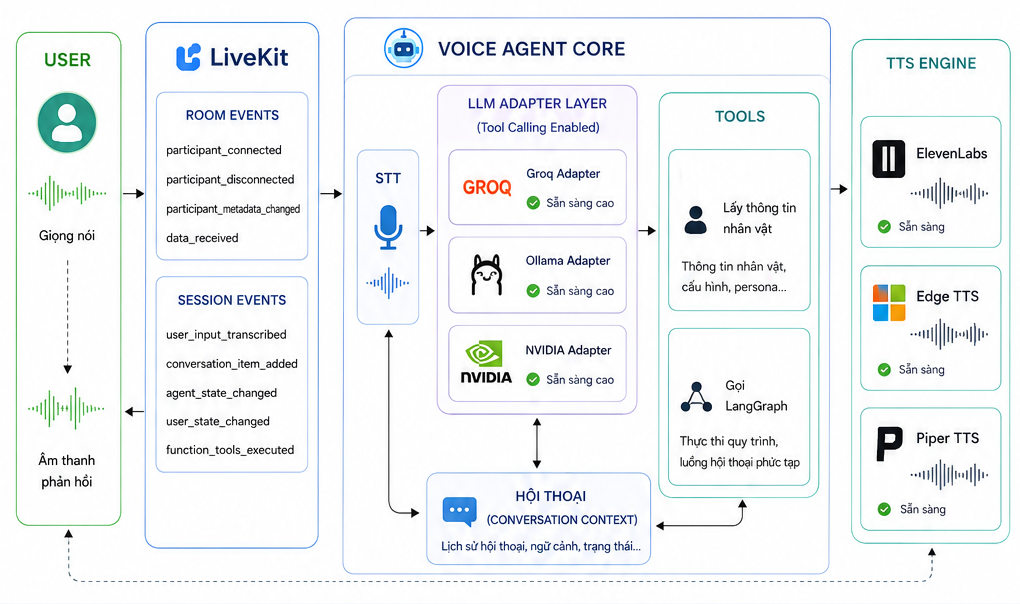
\includegraphics[width=0.99\textwidth]{pictures/voice-livekit-overview.png}
\caption{Sơ đồ tích hợp LiveKit đàm thoại giọng nói}
\end{figure}

Các sự kiện của LiveKit được hệ thống Voice Agent tiếp nhận và xử lý:

\subparagraph{Sự kiện phòng (Room Events)}

Quản lý vòng đời kết nối và sự hiện diện của người dùng trong phòng đàm thoại:

\begin{itemize}
\item \textbf{\texttt{participant\_connected}}: Kích hoạt khi người dùng tham gia vào phòng đàm thoại thành công. Hệ thống tự động gọi hàm chủ động phát giọng nói chào hỏi người dùng
(Lần đầu kết nối:
\texttt{WELCOME\_MESSAGE} = \enquote{Xin chào, tôi là trợ lý pháp luật. Bạn có cần tôi giúp đỡ gì không?},
các lần kết nối lại sau đó:
\texttt{REJOIN\_MESSAGE} = \enquote{Chào mừng bạn đã quay trở lại. Bạn có cần tôi giúp đỡ gì không?}).

\item \textbf{\texttt{participant\_disconnected}}: Kích hoạt khi người dùng rời khỏi phòng hoặc bị ngắt kết nối đột ngột.

\item \textbf{\texttt{participant\_metadata\_changed}}: Lắng nghe sự thay đổi siêu dữ liệu (metadata) từ phía người dùng để cập nhật cấu hình giọng đọc, nhân vật mới một cách tức thời.

\item \textbf{\texttt{data\_received}}: Nhận dữ liệu truyền qua kênh data channel (thường là tin nhắn văn bản định dạng JSON). Cho phép nhà phát triển (developer) gửi tin nhắn văn bản thay cho âm thanh nói để debug luồng xử lý của AI một cách thuận tiện.
\end{itemize}

\subparagraph{Sự kiện phiên thoại (Session Events)}

Quản lý các sự kiện trong luồng đàm thoại giữa người dùng và AI Agent:

\begin{itemize}
\item \textbf{\texttt{user\_input\_transcribed}}: Nhận văn bản sau khi hệ thống Speech-to-Text (STT) chuyển đổi thành công giọng nói của người dùng. Áp dụng bộ lọc \texttt{clean\_transcript} để loại bỏ các đoạn văn bản ảo giác của Whisper, bỏ qua nếu chuỗi rỗng và gọi \texttt{send\_and\_save\_transcript} để hiển thị nội dung văn bản tương ứng lên giao diện UI và lưu vào CSDL.

\item \textbf{\texttt{conversation\_item\_added}}: Kích hoạt mỗi khi có một tin nhắn mới (từ người dùng hoặc AI Assistant) được thêm vào ngữ cảnh trò chuyện. Đối với phản hồi từ AI Assistant, hệ thống tiến hành trích xuất nội dung tin nhắn, kiểm tra và lọc bỏ các bước suy luận trung gian của LangGraph. Khi có câu trả lời cuối cùng, hệ thống gọi \texttt{send\_and\_save\_transcript} để hiển thị trên UI và lưu CSDL.

\item \textbf{\texttt{agent\_state\_changed} và \texttt{user\_state\_changed}}: Theo dõi sự thay đổi trạng thái hoạt động (như Speaking, Listening, Thinking) của cả AI Agent và người dùng để đồng bộ hiển thị trạng thái động trên UI.

\item \textbf{\texttt{function\_tools\_executed}}: Kích hoạt khi AI Agent quyết định gọi một công cụ bên ngoài (Function/Tool Calling) thành công.
\end{itemize}

Bộ lọc làm sạch văn bản \texttt{clean\_transcript} xử lý loại bỏ ảo giác trong văn bản dịch từ giọng nói:

\begin{figure}[H]
\centering
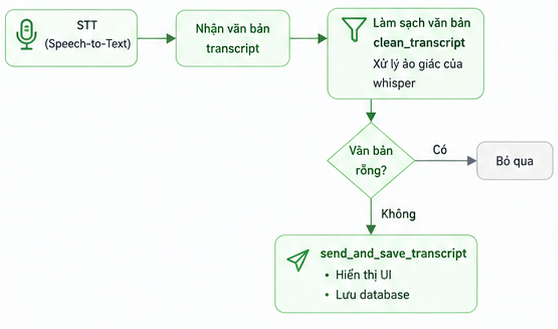
\includegraphics[width=0.99\textwidth]{pictures/voice-clean_transcript.png}
\caption{Bộ lọc làm sạch văn bản clean\_transcript}
\end{figure}

Thông tin log terminal khi AI thực thi công cụ lấy thông tin nhân vật thành công:

\begin{figure}[H]
\centering
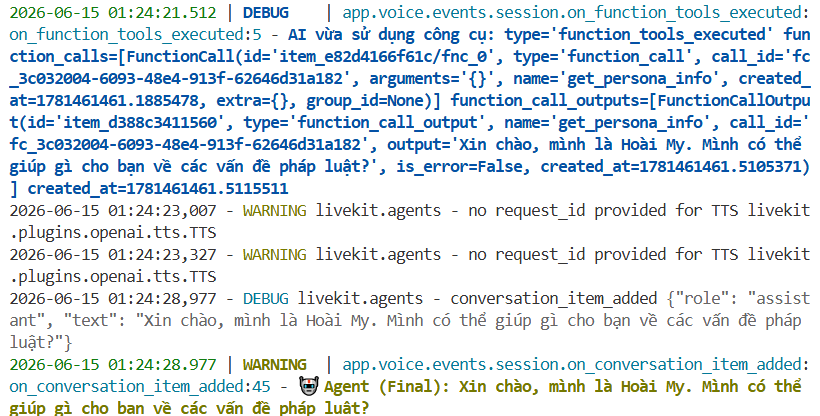
\includegraphics[width=0.95\textwidth]{pictures/voice-get-persona-terminal.png}
\caption{Terminal log của việc gọi công cụ lấy thông tin nhân vật}
\end{figure}

Nhà phát triển gửi thông tin văn bản qua data channel mà không cần nói âm thanh:

\begin{figure}[H]
\centering
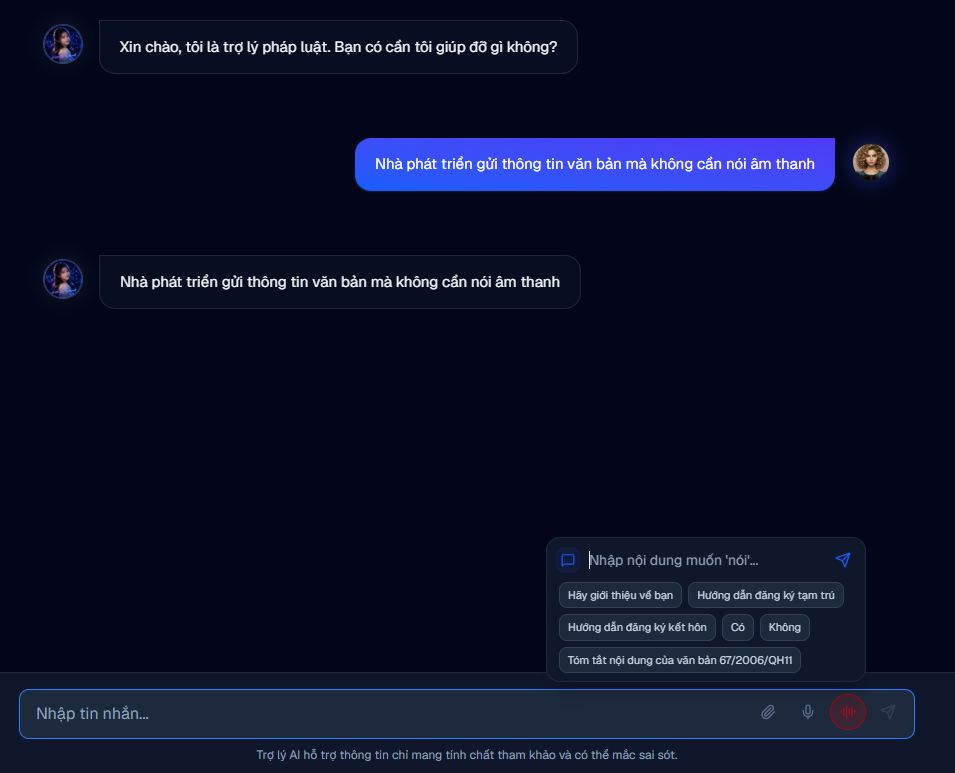
\includegraphics[width=0.9\textwidth]{pictures/voice-developer-send-text.png}
\caption{Nhà phát triển gửi tin nhắn văn bản thay giọng nói để debug}
\end{figure}

% AI Agent sử dụng công cụ lấy thông tin nhân vật từ hệ thống:

\begin{figure}[H]
\centering
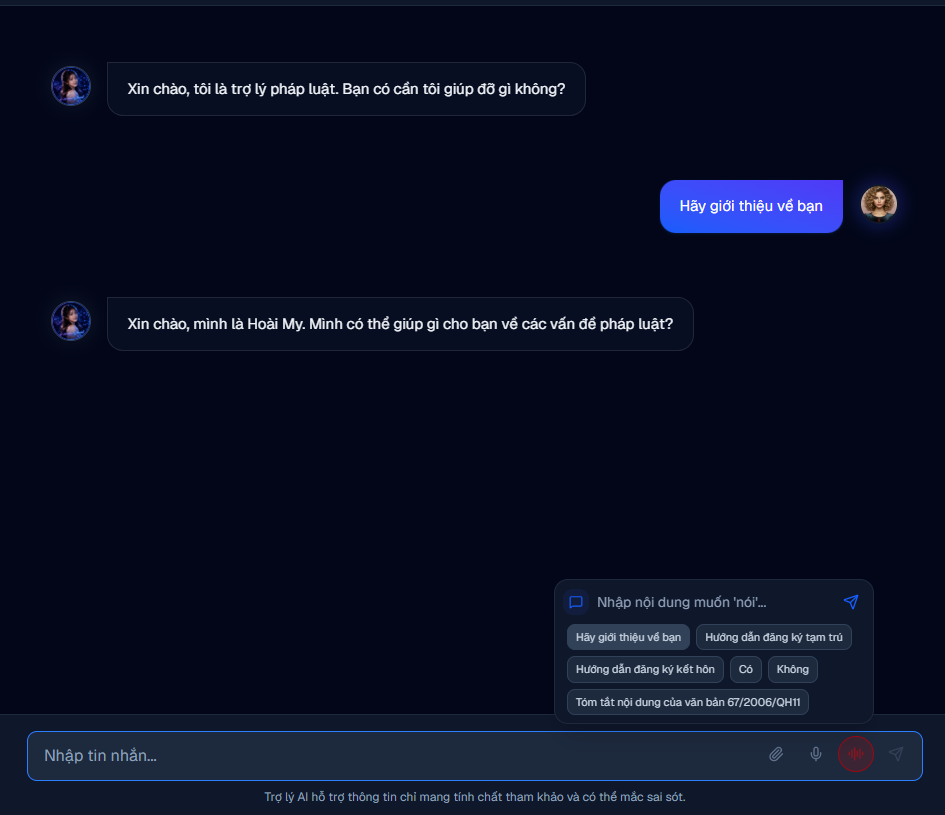
\includegraphics[width=0.9\textwidth]{pictures/voice-get-persona-ui.png}
\caption{Giao diện lấy thông tin nhân vật}
\end{figure}

\paragraph{Cơ chế lập lịch dọn dẹp dữ liệu}

Vì tính năng xóa trò chuyện và thu hồi liên kết chia sẻ trong hệ thống sử dụng cơ chế \textbf{xóa mềm (soft delete)} để đảm bảo tính an toàn dữ liệu và tối ưu hiệu năng của các giao dịch tức thời, hệ thống triển khai các tác vụ lập lịch định kỳ (cron jobs / scheduler) trên cả \textbf{NestJS} và \textbf{Python} để dọn dẹp triệt để các dữ liệu đã bị xóa sau thời gian lưu trữ quy định.

\subparagraph{Phía dịch vụ trò chuyện (NestJS - code-conversation-service)}
NestJS sử dụng module \texttt{@nestjs/schedule} để quản lý các cron jobs dọn dẹp các bản ghi không còn hoạt động quá \textbf{30 ngày}:
\begin{itemize}
\item \textbf{\texttt{ChatCleanupCron}}: Tìm và xóa vĩnh viễn các bản ghi Chat có \texttt{isActive = false} và thời gian cập nhật cách hiện tại từ 30 ngày trở lên. Chu kỳ chạy: Mỗi ngày vào lúc nửa đêm (môi trường production) hoặc mỗi 10 phút (môi trường development).
\item \textbf{\texttt{ShareCleanupCron}}: Tìm và xóa vĩnh viễn các bản ghi liên kết Share có \texttt{isActive = false} (hoặc đã bị thu hồi) quá hạn 30 ngày. Chu kỳ chạy: Mỗi ngày vào lúc nửa đêm (môi trường production) hoặc mỗi 10 phút (môi trường development).
\end{itemize}

\subparagraph{Phía dịch vụ chatbot (Python - code-chatbot-service)}
Python sử dụng \texttt{APScheduler} (\texttt{AsyncIOScheduler}) chạy nền tích hợp trong vòng đời (lifespan) của ứng dụng để tự động dọn dẹp CSDL lưu trữ lịch sử:
\begin{itemize}
\item \textbf{\texttt{run\_chat\_cleanup}}: Xóa vĩnh viễn các bản ghi Chat trong CSDL chatbot có trạng thái \texttt{is\_active = False} quá hạn 30 ngày. Chu kỳ chạy: Mỗi ngày lúc 12:00 trưa (môi trường production) hoặc mỗi 10 phút (môi trường development).
\item \textbf{\texttt{run\_share\_cleanup}}: Xóa vĩnh viễn các bản ghi Share trong CSDL chatbot có trạng thái \texttt{is\_revoked = True} quá hạn 30 ngày. Chu kỳ chạy: Mỗi ngày lúc 12:00 trưa (môi trường production) hoặc mỗi 10 phút (môi trường development).
\end{itemize}
